\chapter{Asset Administration Shell in RAMI 4.0} \label{chap:aas-and-rami}
The previous chapter \ref{chap:basics} described the vertical axis of \ac{RAMI4.0}, which provides insights about the information stored about an asset in \ac{RAMI4.0}. The exchange of information between the layers either takes place within the layer or between neighboring layers. As mean for exchanging information between the layers the \ac{I4.0} component with its \ac{AAS} was introduced. This chapter goes into detail about the \ac{AAS}, works out the characteristic features and classifies the \ac{AAS} in \ac{RAMI4.0}.


\section{General Aspects} \label{sec:assetadministrationshell}
As outlined in chapter \ref{sec:digitaltwin}, the \ac{AAS} is the realization of the \ac{DT} in the context of \ac{I4.0} and contains all relevant data and functions necessary to represent the physical asset in the information world. Figure \ref{fig:structureaas} shows the \ac{AAS} with its structure and characteristic features.

\begin{figure}[h]
\centering
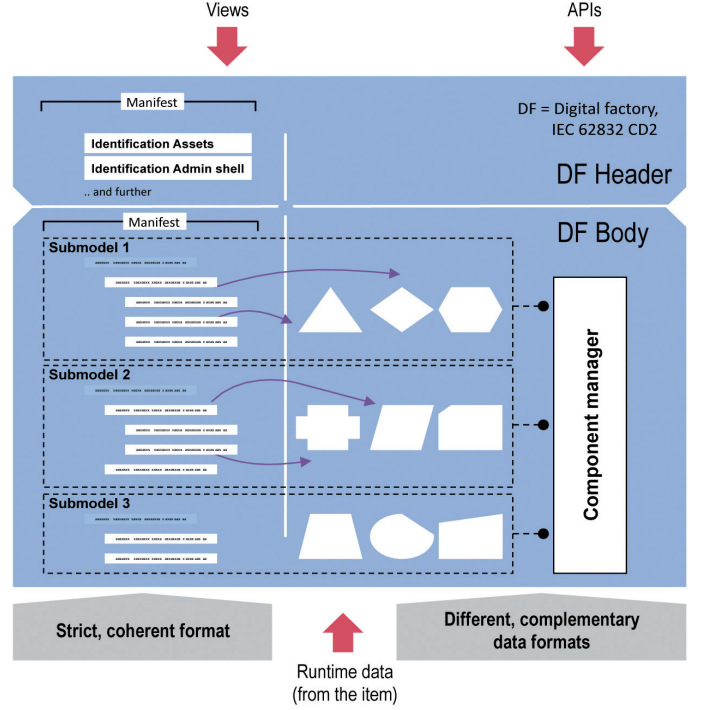
\includegraphics[scale=0.8]{content/pictures/structure_aas_zvei.png}
\caption{Structure of the Asset Administration Shell}
\source{\cite[p. 5]{Koschnick2016Beispiele4.0-Komponente-Basisteil}}
\label{fig:structureaas}
\end{figure}

The \ac{AAS} consists of two parts: The manifest and the component manager. The manifest contains metadata regarding the \ac{I4.0} component, such as a global unique identifier that can be used to identify the \ac{I4.0} component in the value chain. In addition, the metadata provides information whether the \ac{I4.0} component is of type or instance according to the life cycle \& value stream axis in \ac{RAMI4.0}. The component manager provides the uniform interface of the \ac{AAS}, through which the essential properties and functions of the asset can be realized. The goal of the \ac{AAS} is to accommodate as many application scenarios and use cases as possible, so that a variety of different data and functions can be provided \cite[p. 25]{Adolphs2016StructureComponent}. Complex machines, plants and components often consist of several thousand properties in different variants and offer a multitude of functionalities. To group the properties and functions according to their use case, they are represented in submodels within the \ac{AAS}. A submodel describes exactly one property or function of the \ac{I4.0} component in a semantically uniform way. A submodel can model general aspects of the asset or specialized capabilities such as drilling, milling or analytical aspects used for predictive maintenance \cite[p. 23]{Belyaev2021ModellingECLASS}. By encapsulating the properties and functions in independent submodels, the integration of the \ac{I4.0} component in \ac{SOA} is made possible. This way, other \ac{I4.0} components can use the component manager of the \ac{AAS} to query exactly the property or call the function that is needed \cite[p. 6]{Koschnick2016Beispiele4.0-Komponente-Basisteil}, without implementing the full functionality of the asset.

A central vision of \ac{I4.0} is that components can communicate autonomously with each other and make decisions based on contextual information. Although the \ac{AAS} provides a way to query data for different use cases using the component manager, the received data is not directly machine-interpretable nor direct inferences for other components are possible. An explicit knowledge representation in the form of semantic referencing is necessary. For this reason, the \ac{AAS} offers the possibility to reference individual functions and properties of submodels with concept descriptions. Concept descriptions contain the meaning of a property or function of the submodel with all its elements \cite[p. 26]{Bedenbender2019VerwaltungschalePraxis}. Through the exchange of concept descriptions, two components with no previous knowledge of each other's type and interaction models can interact with each other autonomously. To illustrate the structure of a submodel element and the necessity of concept descriptions, Table \ref{tab:rotationspeedex} shows an exemplary submodel element for a property rotation speed of a motor taken from \citet[p. 26]{Belyaev2021ModellingECLASS} \footnote{The table presents the essential properties in a simplified form for better understanding and makes no claim to completeness. A complete example of a submodel including different elements can be seen in \cite[p. 146]{Bader2020Details3.0RC01}}. The value 200 is the expression defined in the submodel. Without the reference to the concept description, it is not immediately clear that this value is the maximum rotation speed of the motor. By referencing the concept description, other components in the system are able to make decisions or perform further calculations. In this example, there could be another component in the system that continuously monitors the rotation speed. Using the \textit{MaxRotationSpeed} property, this component could regulate the rotation speed by continuously comparing the two values. While the functionality as such is not new, however the components are interchangeable and manufacturer independent as long as they are able to interpret and calculate the values based on the submodel. \citet[p. 4]{Lastra2006SemanticRoadmap} found that by introducing semantic referencing in \ac{CPS} new or unknown components can be integrated into systems by asking the question "\textit{can it perform process X?}" rather than "\textit{what vendor/model is it?}".

\begin{table}[ht]
    \centering
    \begin{tabular}{|m{4cm}||m{5cm}||m{5cm}|}
    \hline
        \textbf{Property} & \textbf{Description} & \textbf{Value} \\ \hline
        Id & Unique identification of the element & MaxRotationSpeed  \\ \hline
        Kind & Status according to \ac{RAMI4.0} & INSTANCE  \\ \hline
        Category & Meta-information regarding the type of the value & VARIABLE  \\ \hline
        Value & Observed value of the element & 2000   \\ \hline
        ValueType & Data type of the value & Integer\\ \hline
        SemanticId & Reference to the Semantic Dictionary & 18EBD56F6B43D895 \\ \hline
    \end{tabular}
    \caption{Example submodel element for a property MaxRotationSpeed}
    \label{tab:rotationspeedex}
\end{table}

\begin{table}[ht]
    \centering
    \begin{tabular}{|m{4cm}||m{5cm}||m{5cm}|}
    \hline
        \textbf{Property} & \textbf{Description} & \textbf{Value} \\ \hline
        Id & SemanticId that can be assigned to a property of a submodel & 18EBD56F6B43D895 \\ \hline
        ShortName & Semantic Description of the observed value & Maximum Rotation Speed   \\ \hline
        Data type & Data type of the observed value & INTEGER MEASURE \\ \hline
        Unit & Unit of the observed value & 1/min\\ \hline
        Definition & Detailed human interpretable description & Greatest possible rotation speed with which the motor may be operated \\ \hline
    \end{tabular}
    \caption{Example Semantic Description for a property RotationSpeed}
    \label{tab:rotationspeedex}
\end{table}

In addition to semantic referencing, standardization of properties is an important element of the \ac{AAS} to ensure interoperability. In order to establish a high degree of standardization, four types of characteristics for submodels are distinguished \cite[p. 88]{Heidel2017ReferenzarchitekturmodellIndustrie4.0Komponente}: Basic, mandatory, optional and independent characteristics. The basic and mandatory characteristics aim to reflect the highest possible standardization of a single aspect or capability of an asset. By doing so, individual software solutions do not have to be developed for every single use case and solutions can be used across industries. Optional characteristics are standardized, but not essential to the operation of the asset. Independent characteristics are vendor-specific and therefore neither mandatory nor standardized. 

In order to show the practical implementation as well as the advantages of standardization and semantic referencing in concrete terms, two examples are presented below:

\begin{itemize}

    \item [] \textbf{Digital Nameplate} An example of how to model a general aspect of an asset using a submodel is provided by the digital nameplate. The digital nameplate was developed by the \ac{ZVEI} to provide all legally required information and labeling for the distribution as well as the use of an asset in a digital and standardized form. The starting point of the development was the increasing amount of information and documentation that manufacturers have to provide when selling and operating an asset. In order to sell an asset, manufacturers are required to affix a nameplate to the asset that provides key product usage and classification information for different stakeholders. To cope with the growing amount of mandatory information, taking into account labeling requirements for international sales, manufacturers moved to provide extensive paper documentation when selling the asset. The implementation and maintenance of the documentation causes high costs and efforts \cite[p. 1]{ZVEI2020DasVernetzt}. In order to reduce the effort and cost of maintenance, product documentation as well as services regarding the asset along the entire life cycle can be made available digitally in a submodel of the \ac{AAS}. For this purpose, the manufacture places a QR-code on the asset, which can be scanned using a QR-code-reader to query the related information, documentation and services for the asset. To ensure interoperability, manufacturers are obliged to indicate in the submodel at least the manufacturer's name, its address, product name as well as product type, serial number, country and year of manufacture. This kind of standardization allows a wide range of use cases to be realized: Using the digital nameplate, the inventory of components of a shop floor can be recorded directly in the \ac{ERP} or the product can be automatically checked during customs inspection \cite[p. 4]{ZVEI2020DasVernetzt}
    
    \item [] \textbf{Predictive Maintenance} The use case presented in the following builds on the one described in chapter \ref{fig:valuenetworksi40}. The author's goal is to implement a technology independent approach to predictive maintenance using the \ac{AAS} and its submodels. By describing the functionalities of a predictive maintenance system in a generic way without its concrete implementation, functionalities among different assets and components of both IT and OT can easily be assigned. Since the  \ac{AAS} is a vendor independent digital representation, the predictive maintenance system can be applied to a variety of manufacturers and assets, given that the appropriate submodels are made available in the \ac{I4.0} component. The realization of the predictive maintenance system via the \ac{AAS} was carried out by identifying the main elements of a predictive maintenance system: data acquisition, data processing and maintenance decision making \cite[p. 4]{Cavalieri2020AShell}. In a second step, nine logical blocks were derived on the basis of the main elements, which model the general properties and functionalities used in the  predictive maintenance system. These are for example the measured value, its transformation as well as the calculation of mean values. The logical blocks were then mapped in two submodels \textit{condition monitoring} and \textit{maintenance}. The submodel \textit{condition monitoring} combines data acquisition and data processing properties and functionalities. The submodel \textit{maintenance} maps the main element decision making. The prediction function itself was not represented in a submodel because the authors found it  difficult to generalize \cite[p. 10]{Cavalieri2020AShell}. Proof of practical interoperability was provided by implementing the outlined solution on 100 milling machines from different manufacturers. The authors were able to show that the process of data collection, harmonization and evaluation for predictive maintenance could be standardized to such an extent that it could be applied to different manufacturers' machines without any adoption of the submodels  \cite[p. 17]{Cavalieri2020AShell}.  
\end{itemize}

In general, it can be assumed that not every component within a system can directly be equipped or described with an \ac{AAS}. This can have both, economic and technical reasons \footnote{A good classification about when and for which components it makes sense to provide a separate \ac{AAS} is given in this podcast by Bosch Rexroth \cite{Noll2021WasRexroth}.}. Depending on how the \ac{I4.0} component is implemented, the \ac{AAS} can take different forms. To this end, the role of the \ac{AAS} in value networks is considered, as well as the method of distribution and the composition of the \ac{AAS}:

\begin{itemize}
    \item [] \textbf{Role in value networks} A distinction is made between an active and passive \ac{AAS}. A passive \ac{AAS} only provides their information in a standardized format via file or \ac{API} and therefore provides read-only access to the properties in the submodels. In contrast, an active \ac{AAS} can communicate directly with other \ac{AAS} in the system based on the \ac{I4.0} language, described in chapter \ref{sec:interaction-i4.0-comp} \cite[p. 19]{Bedenbender2019VerwaltungschalePraxis}. For this purpose, the functionalities of the asset are described in separate submodels alongside the properties and can be addressed and executed with the help of the component manager. In this process, active \ac{AAS} carry out their tasks  and requests without a central control unit; rather, the \ac{AAS} in the system contact each other independently. 
    
    \item [] \textbf{Distribution} The distribution of the \ac{AAS} can be done in two ways. The \ac{AAS} can be stored directly on the asset or distributed in a higher level system. Assets that have \ac{I4.0} compatible communication capabilities can provide the \ac{AAS} itself for example via \ac{OPCUA}. It is also possible to make the \ac{AAS} available via a \ac{SBC} such as a Raspberry Pi, for assets that do have a controller but do not have direct \ac{I4.0} compatible communication capabilities. The communication would then be realized exclusively via the respective \ac{SBC}.  For assets that do not have \ac{I4.0} compatible communication capabilities and do not have a control unit, the provisioning and communication of the \ac{AAS} is realized via a central repository. The central repository can be the \ac{ERP}-System or a dedicated database, that stores all the submodels of the \ac{AAS} \cite[p. 18]{Bedenbender2019VerwaltungschalePraxis}.
    
    \item [] \textbf{Composition} In general, two types of composition are distinguished. An asset can occur through one or more \ac{AAS}. This assumes that the \ac{AAS}s represent the various aspects of \ac{RAMI4.0} and relate to each other. However, one \ac{AAS} can also represent multiple assets. This is the case when multiple individual assets are combined into a composite \ac{I4.0} component. For example, when a manufacturer sells an entire milling center, where the individual elements of the milling center provide their own \ac{AAS}, which are referenced then in the \ac{AAS} of the milling center. \cite[p. 29]{Adolphs2016StructureComponent}.
 \end{itemize}

\section{Interaction between I4.0 components} \label{sec:interaction-i4.0-comp}
The presented use cases of digital nameplate as well as predictive maintenance describe the role of passive \ac{AAS} in value networks. However, to realize the vision of \ac{I4.0}, individual \ac{AAS} must communicate autonomously with each other and therefore be active. Based on the use case of plug and produce, the interaction model of \ac{I4.0} components and thus active \ac{AAS} and its characteristics will be presented in the following. As outlined in chapter \ref{chap:introduction} companies are moving towards \ac{SOA} to increase the flexibility of production to realize order-controlled production. This is necessary because in an \ac{I4.0} compliant system no fixed allocation of production resources to the product being produced can be made in advance. Instead, production resources must be selected during runtime and configure themselves dynamically according to the given job \cite[p. 6]{Bock2016Weiterentwicklung4.0-Komponenten}. To realize this, the production resources under consideration for executing the needed production steps must interact with each other via the standardized interface of the \ac{AAS}. The goal of the interaction in plug and produce is to determine (a) which of the available resources can best meet the requirements for a given job in terms of cost, time and quality, (b) carry out the self-commissioning of the selected components, as well as to carry out the production process. To this end, the business processes as well as the requirements in terms of cost, time and quality are defined in the business layer of \ac{RAMI4.0} and provided in the functional layer by the corresponding services. 

The interaction to define the production process in plug and produce consists basically of two essential steps: Capability and feasibility checking. Capability checking describes the process of determining whether a resource within a value network is suitable in general for executing a given job \cite[p. 6]{Bayha2020DescribingComponents}. For this purpose, a request from a service in the functional layer in \ac{RAMI4.0} is sent to the available \ac{AAS} in the value network. Based on the request, the individual components decide, whether they can execute the order by matching the request parameters with their properties in the respective submodel and respond with a positive or negative answer to the service \cite[p. 20]{Bock2016Weiterentwicklung4.0-Komponenten} \footnote{\citet[p. 22]{Bock2016Weiterentwicklung4.0-Komponenten} present an example illustration of the interaction between two \ac{I4.0} components for the negotiation of a production order.}. The final decision about which component will execute the given job is finally made by the requesting service in the functional layer based on the criteria defined in the business layer. While capability checking focuses on the functionality of the individual components, feasibility checking assures that the selected component in the value networking is able to perform the task according to the specified requirements by checking various conditions \cite[p. 6]{Bayha2020DescribingComponents} \cite[p. 15]{Bock2016Weiterentwicklung4.0-Komponenten}. In case of a robot that moves objects from A to B, this could be the condition that the object to be moved is actually located at location A by another component or service involved in the process.

An important requirement for making production more flexible and therefore realize a \ac{SOA} is, that services within an \ac{SOA} are loosely coupled and not controlled by a central instance. For this reason, each service or \ac{I4.0} component within an \ac{I4.0} system manages its status by itself in a submodel. Status in this context refers to the operating status, for example, whether the \ac{I4.0} component is currently busy or free to accept new offers \cite[p. 38 ]{Epple2018BaSysAufbaus}. This is important in that way, as this allows any other service or component within the \ac{I4.0} system to query the status of other components and make its own decision based on it. Depending on the use case, an \ac{I4.0} component can have different status \cite[p. 30]{Epple2018BaSysAufbaus}. To illustrate this, the commissioning process in the plug and produce use case will be explained based on the work of \citeauthor{Schweizer2021ProcessSystems} The goal of the commissioning process in a plug and produce system is, that the involved components in a production process configure themselves automatically without manual intervention, so that complexity and the error rate can be reduced \cite[p. 244]{Schweizer2021ProcessSystems}. While in an Industrie 3.0 system, the steps for commissioning are mainly in the engineer's head, in an \ac{I4.0} system they are stored as process models in the submodel \textit{PlugAndProduce} of the components \ac{AAS} \cite[p. 246]{Schweizer2021ProcessSystems}. Each of the components in the system defines therefore its own possible states, which must be passed during the commissioning as well as its current state. In the present use case, the states, each component must go through are power-free operation, low-power operation, full-power operation, and production operation. The commissioning of the entire system then takes place in that way, that the individual components in the system go through their commissioning sequences independently. By doing so, the components inform each other about the current status and the current commissioning step in a cooperative manner. \cite[p. 252]{Schweizer2021ProcessSystems}. By exchanging messages about changes and current states, complex dependencies between different components can be realized. For example, component 1 can wait with its commissioning process until component 2 has transitioned to a required status or finished its commissioning process.       

As outlined in the example of the commissioning process, the \ac{AAS} and the interaction of the components allow the implementation of complex business processes in a \ac{SOA}. However, in order to be able to communicate both vertically and horizontally as part of an I4.0 system, a uniform set of rules must be defined for communication so that messages can be exchanged between machines in a readable and interoperable manner. With the help of the \ac{I4.0} language, a set of grammar and rules are defined to make this possible. The \ac{I4.0} language defines three essential components for realization. These are vocabulary, message structure, and interaction protocol \cite[p. 12, figure 8]{Bock2016Weiterentwicklung4.0-Komponenten}, which are described in the following.

\begin{itemize}
    \item [] \textbf{Vocabulary} A distinction is made between basic vocabulary and domain-specific vocabulary \cite[p. 12]{Bock2016Weiterentwicklung4.0-Komponenten}. Basic vocabulary describes all the properties and functionalities of an asset that can be used to describe the asset regardless of a specific scope. For example, the localization of an asset. Domain-specific vocabulary describes the properties and functions required for a specific application area. The main elements of the vocabulary are the properties of the \ac{AAS}, which are stored in the submodels.
    \item [] \textbf{Message Structure} Message basically consist of an identification and data area. The identification area is used for the identification of the sender and receiver as well as for the conversation and message itself. The data area consists of the action and the associated data elements, which is received, evaluated and executed by the component manager of the \ac{AAS} \cite[p. 17]{Bock2016Weiterentwicklung4.0-Komponenten}.
    \item [] \textbf{Interaction Protocol} An interaction protocol arise from a sequence of messages exchanged between \ac{I4.0} components to accomplish a task and the submodels involved to perform the task \cite[p. 13]{Bock2016Weiterentwicklung4.0-Komponenten}.
\end{itemize}

Figure \ref{fig:interaction-concept-i40} illustrates the relationship between the individual elements of the \ac{I4.0} language. The vocabulary is defined in the submodels and the interaction between the individual \ac{AAS}s takes place by means of messages. The autonomous interaction of the components takes place via the interaction protocols, which specify the sequence of the task. The component manager, which was introduced in chapter \ref{sec:assetadministrationshell}, receives the message, executes the required action within the submodel and communicates the decision of the action via the interaction protocol.

\begin{figure}[h]
\centering
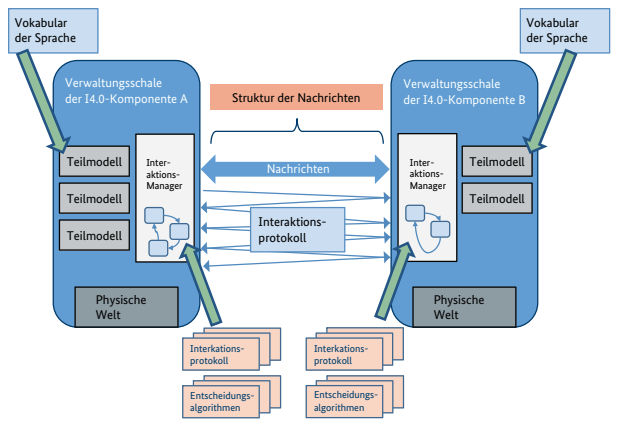
\includegraphics[scale=0.7]{content/pictures/interaction_i40_components.png}
\caption{Interaction concept of Industry 4.0 components in RAMI 4.0}
\source{\cite[p. 16]{Vialkowitsch2018VokabularI4.0-Sprache}}
\label{fig:interaction-concept-i40}
\end{figure}

\section{Classification in RAMI 4.0}

Using the outlined use cases it becomes clear, that the type of asset belonging to a \ac{I4.0} component determines its location in \ac{RAMI4.0}. In order to show the relationship between the \ac{AAS} and \ac{RAMI4.0}, the \ac{AAS} is to be classified in the six layers of \ac{RAMI4.0}. The aim of the classification is to summarize the forms of the \ac{AAS} and to highlight the associated characteristics in \ac{RAMI4.0}.

In case of the digital nameplate, the role of the \ac{AAS} in the value network is passive and therefore extends until the information layer in \ac{RAMI4.0}. Figure \ref{fig:aas-until-info-layer} graphically shows the relationship between the \ac{AAS} and \ac{RAMI4.0}. The data of the respective \ac{I4.0} component is manifested in the \ac{AAS} in the form of submodels using properties. These are stored and prepared in the information layer, enabling interoperable access by the function and business layer. Passive \ac{AAS} do not have any capabilities or functionalities and therefore have no representation in the functional or business layer. Hence, \ac{I4.0} components without a functional and business layer only contain the option for data retrieval and persistence. They can neither execute activities nor synchronize with other components in a system by means of message exchange.
\begin{figure}[h]
\centering
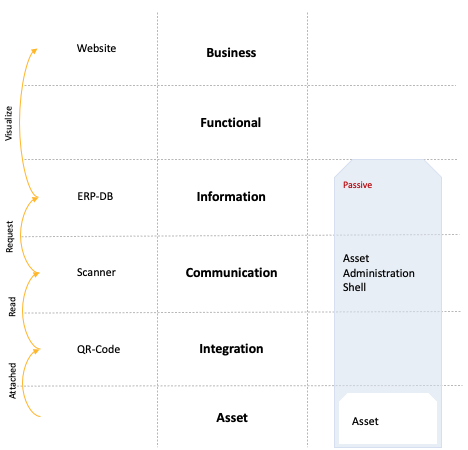
\includegraphics[width=.45\textwidth]{content/pictures/aas_rami_v1.png}
\caption{Asset Administration Shell until Information Layer}
\source{Own illustration}
\label{fig:aas-until-info-layer}
\end{figure}

The \ac{AAS} in the use case of predictive maintenance as well as plug and produce have a representation in the functional layer. The latter also includes an explicit representation in the business layer. Figure \ref{fig:aas-until-func-and-bizz-layer} graphically classifies the \ac{AAS} in \ac{RAMI4.0}, where (a) shows the use case of predictive maintenance and (b) the use case of plug and produce. Depending on whether the \ac{AAS} in the use case of predictive maintenance makes independent decisions, the \ac{AAS} are to be classified as active in regards to their role in value networks. The functionality for decision making is manifested in the business layer for active \ac{AAS}. It should be noted in both cases, that the information layer is essential for the functional layer. Without the data stored in the information layer and made available via the standardized interface of the \ac{AAS}, interoperable functionalities of the assets cannot be designed and implemented in the functional layer. The business layer provides the decision logic for executing the business and production processes based on defined business models. This includes, for example, the conditions for cost, quality and time when selecting production resources during capability checking. An important characteristic of active \ac{AAS} is, that it stores its own operating state. This is stored in a defined submodel in the information layer.

\begin{figure}[h]
\centering
\subfigure[]{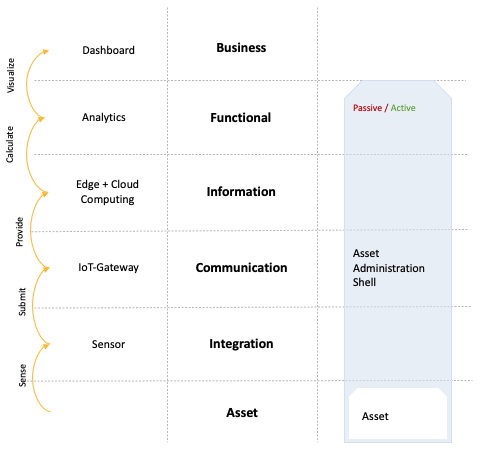
\includegraphics[width=.45\textwidth]{content/pictures/aas_rami_v2.png}}
\subfigure[]{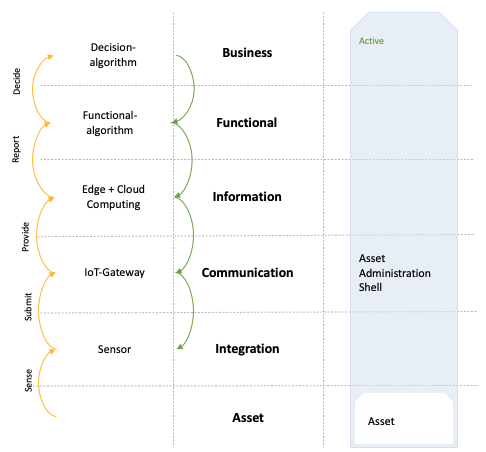
\includegraphics[width=.45\textwidth]{content/pictures/aas_rami_v3.png}}
\caption{(a) Asset Administration Shell until Functional Layer, (b) Asset Administration Shell until Business Layer}
\source{Own illustration}
\label{fig:aas-until-func-and-bizz-layer}
\end{figure}

For the type of distribution of an \ac{AAS} it can be said, that it is irrelevant whether the \ac{AAS} is provided by the asset itself, or by a central repository. However it should be noted, that for assets providing the \ac{AAS} by themselves, care must be taken to ensure \ac{I4.0} compliant communication capabilities. Otherwise, additional hardware must be attached to the asset, which can be used to realized the \ac{I4.0} compliant communication.  

For the composition of the \ac{AAS} different characteristics can be observed in the presented use cases. According to \ac{RAMI4.0}, an asset can be represented by several \ac{AAS}. This is done on the basis of the lifecycle phases \textit{type} and \textit{instance} or in order to represent different aspects of \ac{RAMI4.0} such as design, production or operation. Likewise, an \ac{AAS} can also contain or reference further \ac{AAS}. The composition does not play a significant role for the digital nameplate, as the provision of one \ac{AAS} per asset is recommended. Two different forms of composition can be observed in the use cases of predictive maintenance and plug and produce. In the case of plug and produce, each individual component in the system is described by its own \ac{AAS}. The overall system itself is being represented by an \ac{AAS} which references the individual \ac{AAS} of the components in the system \footnote{A graphical representation of this composition can bee seen in \citet[p. 246, figure 3]{Schweizer2021ProcessSystems}}. This type of composition has advantages especially for plug and produce, so that components in the system can individually be addressed and exchanged flexibly as the configuration is carried out by the component itself. In case of predictive maintenance, the type of composition cannot be derived directly from the paper of \citeauthor{Cavalieri2020AShell}. To ensure the best implementation, the following composition would be suitable: One \ac{AAS} is modeled for the entire milling station, which stores all properties and functionalities of the contained components. Although this can make the modeling of the \ac{AAS} complex in terms of submodels and bill of material, unnecessary hardware regarding networking and computation can be reduced. Similarly, network latencies can be reduced, making access to the information and functionalities in the submodels by other components more efficient. Likewise, the provision of the \ac{AAS} is simplified.